\documentclass{article}

\usepackage{microtype}
\usepackage{graphicx}
\usepackage{subcaption}
\usepackage{booktabs}
\usepackage{amsmath}
\usepackage{amssymb}
\usepackage{mathtools}
\usepackage{hyperref}
\newcommand{\theHalgorithm}{\arabic{algorithm}}
\makeatletter
\def\input@path{{icml2026/}}
\makeatother
\usepackage[accepted]{icml2026}
\makeatletter
\renewcommand{\ICML@appearing}{\textit{Final project report. New York University, 2026.}}
\makeatother
\renewcommand{\ttdefault}{cmtt}

\icmltitlerunning{Self-Supervised Representations for Active Matter}

\begin{document}

\twocolumn[
\icmltitle{Self-Supervised Spatiotemporal Representations for Active Matter Parameter Regression}

\icmlsetsymbol{equal}{*}

\begin{icmlauthorlist}
  \icmlauthor{Abhinay Krishna Bodi (ab11958)}{equal,nyu}
  \icmlauthor{Georgios Ioannao (gi2100)}{equal,nyu}
\end{icmlauthorlist}

\icmlaffiliation{nyu}{New York University}
\icmlcorrespondingauthor{Abhinay Krishna Bodi}{ab11958@nyu.edu}
\icmlcorrespondingauthor{Georgios Ioannao}{gi2100@nyu.edu}
\icmlkeywords{Self-supervised learning, physical simulation, active matter, JEPA, ConvNeXt, kNN regression}
\hypersetup{pdfsubject={Final project report. New York University, 2026}}

\vskip 0.3in
]

\printAffiliationsAndNotice{\icmlEqualContribution}

\begin{abstract}
We study self-supervised representation learning for the \texttt{active\_matter} dataset from The Well, where the final task is to recover the physical parameters $\alpha$ and $\zeta$ from frozen video embeddings using only a linear probe or k-nearest-neighbor regression. We compare three completed training paths: a JEPA-style ConvNeXt encoder regularized with VICReg, a larger SigReg-based JEPA variant that exposed collapse and evaluation pitfalls, and a final CNext-U-Net future-frame forecaster trained from scratch at $96\times 96$ resolution. The final encoder uses a forecasting decoder only during pretraining; downstream evaluation freezes the bottleneck encoder and exports trajectory-level pooled embeddings. The selected average-pooled model achieves normalized test mean MSE $0.1043$ with a linear probe and $0.0989$ with kNN regression, improving over the JEPA/VICReg baseline at both $224\times224$ ($0.2485$ / $0.2709$) and a resolution-matched $96\times96$ rerun ($0.4260$ / $0.3865$). Our analysis shows that the largest gains come from replacing fragile distribution matching with a direct physical forecasting objective.
\end{abstract}

\section{Introduction}

Learning representations from physical simulations without labels is attractive because high-dimensional spatiotemporal fields are often easy to generate or store, while downstream physical parameters may be sparse, expensive, or intentionally withheld during representation learning. The project setting follows this regime: train an encoder on unlabeled active-matter trajectories, freeze it, and evaluate whether the resulting embedding predicts two physical parameters, active dipole strength $\alpha$ and steric alignment $\zeta$, using only a single linear layer or kNN regression.

The core challenge is that a low pretraining loss does not necessarily imply a useful downstream embedding. Joint-embedding predictive methods can collapse to low-dimensional solutions if the prediction target is too easy or the anti-collapse mechanism is too weak. Conversely, reconstruction objectives can learn low-level field statistics that may not align with the downstream parameter geometry. Our work therefore emphasizes not only the final MSE, but also the training dynamics, embedding-space diagnostics, and failure modes that led to the final model choice.

We began with a JEPA-style ConvNeXt encoder trained with VICReg \citep{bardes2021vicreg}. This baseline produced healthy, non-collapsed embeddings and achieved a normalized linear-probe test MSE of $0.2485$. We then scaled the encoder and tried a SigReg-style distribution regularizer, motivated by the idea that isotropic embeddings should improve distance-based regression. This run failed: the prediction loss reached near zero by epoch 2, the SigReg term froze, and 62 of 256 embedding dimensions became nearly dead. Finally, we moved to a CNext-U-Net forecaster inspired by ConvNeXt \citep{liu2022convnext} and U-Net-style encoder--decoder architectures \citep{ronneberger2015unet}. This final approach directly predicts the next physical frame from context frames, then discards the decoder and evaluates the frozen bottleneck encoder.

Our main result is that the final CNext-U-Net encoder improves both allowed downstream evaluators: normalized test mean MSE drops from $0.2485$ to $0.1043$ for the linear probe and from $0.2709$ to $0.0989$ for kNN. The strongest result is kNN, which suggests the forecasting objective learned a neighborhood geometry where nearby embeddings share physical parameters, especially $\alpha$.

\section{Related Work}

Recent video self-supervised learning has shown that useful frozen representations can be learned from temporal structure alone. VideoMAE reconstructs heavily masked video tubes and demonstrates that masked video reconstruction can be data-efficient when the pretext task is sufficiently difficult \citep{tong2022videomae}. V-JEPA instead predicts latent video features and motivates our initial JEPA direction because it separates representation learning from pixel-level reconstruction and evaluates frozen backbones on downstream tasks \citep{bardes2024vjepa}. Our final method keeps the frozen-encoder evaluation philosophy, but uses a physical forecasting target because the active-matter labels are parameters of the underlying dynamics rather than object categories.

Forecasting has also been studied as a direct spatiotemporal pretraining signal. PredRNN models future frames with recurrent spatiotemporal memory \citep{wang2017predrnn}, while SimVP shows that a simpler convolutional encoder--translator--decoder trained with MSE can be a strong video-prediction baseline \citep{gao2022simvp}. This motivated our CNext-U-Net design: we use next-frame prediction to force the bottleneck to retain information about dynamics, then discard the decoder and evaluate only the encoder. In contrast to masked autoencoding, which can emphasize spatial inpainting, our objective asks whether recent physical fields contain enough information to predict the next field.

The anti-collapse regularizers in our earlier runs are related to redundancy-reduction SSL. Barlow Twins makes the cross-correlation matrix between two views close to the identity \citep{zbontar2021barlow}, while VICReg separately penalizes representation mismatch, low per-dimension variance, and covariance \citep{bardes2021vicreg}. We chose VICReg first because its variance and covariance terms provide direct diagnostics for collapse in small scientific datasets. The later SigReg-style run tested an isotropic distribution penalty, but its weak weighting failed to move the embedding distribution once the prediction loss had already saturated.

\section{Task, Data, and Evaluation}

\paragraph{Dataset.}
We use the \texttt{active\_matter} dataset from The Well, a benchmark collection of spatiotemporal physical simulations stored in a unified HDF5 format \citep{ohana2024well}. Each sample contains multiple field groups; our loader discovers scalar, vector, and tensor-valued fields under \texttt{t0\_fields}, \texttt{t1\_fields}, and \texttt{t2\_fields}, yielding 11 input channels. The project provides train, validation, and test splits. Representation learning is performed without reading $\alpha$ or $\zeta$ labels; labels are introduced only after the encoder is frozen and embeddings are exported.

The original JEPA/VICReg baseline was trained with $224\times224$ frames. For the final forecaster, we resized frames to $96\times96$. This was a deliberate preprocessing choice after TA clarification that the project did not require a fixed $224\times224$ input size. The $96\times96$ setting reduces the spatial area by about $5.4\times$, making full 50-epoch forecasting feasible while preserving enough spatial resolution for the active-matter field patterns.

\paragraph{Windows versus trajectories.}
The large sample counts used during self-supervised training are window counts, not independent downstream label examples. A single simulation trajectory can produce many overlapping temporal windows, and all of those windows share the same scalar parameters $(\alpha,\zeta)$. For representation learning we use these windows as unlabeled forecasting examples, which increases the number of optimization steps without using labels. For downstream evaluation, however, we report one frozen embedding per simulation trajectory. This matches the parameter-regression protocol because each trajectory has one ground-truth $(\alpha,\zeta)$ pair, and it avoids artificially inflating the linear-probe or kNN training set with many nearly identical windows carrying duplicated labels. The split is fixed before any windowing, so no windows from validation or test trajectories enter representation learning or downstream model fitting.

\paragraph{Representation-learning constraint.}
All encoders are trained from scratch, with no pretrained weights and no external data. During pretraining, \texttt{ActiveMatterWindowDataset} is instantiated with \texttt{include\_labels=False}, so scalar labels are not loaded into the training examples. Validation trajectories are used only to choose checkpoints and hyperparameters. Test labels are used only for final reporting.

For the final CNext-U-Net run, the SSL training loader used \texttt{max\_train\_samples=None}, \texttt{train\_index\_mode=sliding\_window}, and stride 1 on the training split only. This produced 13,475 unlabeled $96\times96$ forecasting windows from the available train trajectories. Validation was not used to update model weights; it was used only for checkpoint selection with one deterministic clip per validation trajectory. Test trajectories were never used during SSL training, checkpointing, hyperparameter selection, or downstream fitting, and were used only for final frozen-encoder evaluation.

\begin{table}[t]
\centering
\caption{Data usage across self-supervised training and downstream evaluation for the final CNext-U-Net run.}
\label{tab:data_usage}
\resizebox{\columnwidth}{!}{%
\begin{tabular}{llrl}
\toprule
Stage & Split used & Count & Meaning \\
\midrule
SSL CNext training & train only & 13,475 & unlabeled sliding windows from train trajectories \\
SSL validation/checkpointing & validation only & 24 & one deterministic validation clip per trajectory \\
Downstream train & train & 175 & one frozen embedding per train trajectory \\
Downstream validation & validation & 24 & one frozen embedding per validation trajectory \\
Final test & test & 26 & one frozen embedding per test trajectory \\
\bottomrule
\end{tabular}
}
\end{table}

\paragraph{Downstream metrics.}
Let $y=(\alpha,\zeta)$ and let $\mu_{\mathrm{train}},\sigma_{\mathrm{train}}$ denote the mean and standard deviation of train labels. Downstream evaluators predict normalized targets
\begin{equation}
  \tilde{y} = (y-\mu_{\mathrm{train}})/\sigma_{\mathrm{train}},
\end{equation}
and we report normalized mean squared error, averaged across $\alpha$ and $\zeta$. We also report per-parameter normalized MSE to diagnose which physical parameter is encoded more clearly. The linear probe is a single affine layer trained on frozen embeddings. The kNN evaluator fits no neural parameters; it searches validation-selected neighbors over frozen train embeddings.

\section{Methods}

\subsection{JEPA/VICReg Baseline}

The first baseline is a joint-embedding predictive architecture in the spirit of I-JEPA \citep{assran2023ijepa}, adapted to full spatiotemporal clips. A ConvNeXt-style encoder maps a 16-frame context clip to a feature map, and a convolutional predictor maps context features to target features. VICReg regularizes the output with similarity, variance, and covariance terms:
\begin{equation}
  \mathcal{L}_{\mathrm{VICReg}}
  = \lambda_s \mathcal{L}_{\mathrm{repr}}
  + \lambda_v \mathcal{L}_{\mathrm{std}}
  + \lambda_c \mathcal{L}_{\mathrm{cov}}.
\end{equation}
We used $\lambda_s=2$, $\lambda_v=40$, and $\lambda_c=2$. This objective is useful in this setting because the variance and covariance terms remain active even when the prediction term becomes small, preventing the encoder from mapping all clips to the same vector.

The baseline encoder has 3.27M parameters. It was trained at $224\times224$ resolution with AdamW, learning rate $5\cdot 10^{-4}$, weight decay $5\cdot 10^{-4}$, bfloat16 automatic mixed precision, and a global batch size of 16. Although training ran for 12 epochs, downstream embeddings were exported from the epoch-5 checkpoint because it had the lowest validation loss. Validation loss decreased from 16.22 at epoch 1 to 8.51 at epoch 5, then increased to 10.27 by epoch 12. Thus, the reported JEPA/VICReg baseline uses validation-based checkpoint selection rather than the final training epoch.

\subsection{ConvNeXt JEPA with SigReg}

The second run tested a larger 9.83M parameter JEPA encoder with a 256-dimensional embedding, an MLP projector, and an MLP predictor. The objective combined prediction loss and a SigReg-style distribution penalty,
\begin{equation}
  \mathcal{L}
  = 0.95\,\mathcal{L}_{\mathrm{pred}}
  + 0.05\,\mathcal{L}_{\mathrm{sigreg}},
\end{equation}
where the regularizer measures deviation from an isotropic Gaussian through randomized one-dimensional projections. We enabled target stop-gradient in the corrected run to break the symmetric collapse path where context and target branches move together.

This experiment was important despite underperforming. It isolated a failure mode: with $\lambda=0.05$, the distribution term was too weak relative to the rapidly solved prediction loss. By epoch 2, prediction loss was already near zero; the encoder then stopped receiving useful pressure to improve its embedding distribution. The SigReg loss stayed frozen around 25.7268 on train and 9.625 on validation for the rest of the run.

\subsection{Auxiliary Masked-Video and Supervised Diagnostics}

In parallel with the final model, we ran diagnostic probes to understand whether the dataset rewards temporal context, channel content, and class separability. These runs were trained from scratch on \texttt{active\_matter}. The supervised ConvNeXt probes used $(\alpha,\zeta)$ labels directly and are therefore not eligible self-supervised submissions; they serve only as label-aware reference points. The VideoMAE-style probes used masked-video reconstruction, varying mask ratio, seed, training length, and the number of frames used at evaluation time \citep{tong2022videomae,he2022mae,xie2022simmim}. We also performed channel zero-out ablations, nearest-centroid classification over the 45 discrete $(\alpha,\zeta)$ combinations, and validation-set CKA comparisons between encoders \citep{kornblith2019cka}. These diagnostics explain the geometry of the task but were not used to choose the final checkpoint or final downstream hyperparameters.

\subsection{Final CNext-U-Net Forecaster}

The final model is a scratch CNext-U-Net forecaster. It uses ConvNeXt-style blocks in an encoder--decoder topology, predicts the next physical frame from a short context, and then discards the decoder for downstream evaluation. The choice is deliberately simple: instead of matching latent targets with a weak distribution regularizer, the model must preserve information sufficient to predict future physical fields.

The input tensor has shape $(B,11,4,96,96)$. We chose a 4-context-frame to 1-target-frame task because it is long enough to expose short-horizon dynamics, but short enough to fit full-field forecasting at $96\times96$ without making the target dominated by long-range uncertainty. We fold time into the channel dimension, giving a 44-channel 2D input, and use a $3\times3$ input projection to 42 channels. The base width of 42 was chosen to use the available parameter budget while keeping the full model far below the 100M-parameter project limit. The encoder has four downsampling stages with channel widths $42,84,168,336,672$ and two CNext blocks per stage; four stages reduce $96\times96$ inputs to a $6\times6$ bottleneck, giving global context without collapsing the spatial grid to a single token. Each CNext block uses a $7\times7$ depthwise convolution, LayerNorm, a four-times-expanded MLP with GELU activation, residual connection, and layer scale. The $7\times7$ depthwise convolution follows ConvNeXt practice: it gives a larger spatial receptive field than a $3\times3$ standard convolution at much lower channel-mixing cost, leaving channel mixing to the MLP. Layer scale stabilizes residual updates in the deeper encoder; we did not use dropout because dense forecasting already supplies a per-pixel training signal, and stochastic feature dropping made less sense for preserving physical fields. The bottleneck is a $672$-channel $6\times6$ feature map. The decoder mirrors the encoder with transposed-convolution upsampling and skip connections, and predicts an output tensor of shape $(B,11,1,96,96)$.

The forecaster takes 4 context frames and predicts the next 1 frame at $96\times96$ resolution. The encoder has 7.34M parameters; the full pretraining model has 18.59M parameters, so both the submitted backbone and the training model are below the required 100M-parameter ceiling. We trained for 50 epochs using AdamW with learning rate $3\cdot10^{-4}$, weight decay $5\cdot10^{-4}$, gradient clipping at 1.0, bfloat16 AMP, and batch size 16. The training set used sliding windows, giving 13,475 unlabeled forecasting examples; validation used one deterministic clip per trajectory, giving 24 validation examples. The best validation checkpoint was epoch 49 with validation MSE $7.72\cdot10^{-4}$ and validation relative MSE $0.00252$.

For embedding export, the encoder is frozen. We use one deterministic 16-frame clip per simulation and apply the 4-frame encoder to all 13 overlapping context windows inside that clip. The resulting bottleneck feature maps are averaged over time windows, then pooled spatially. We evaluated average pooling, max pooling, and average+max concatenation; validation selection chose average pooling as the final export, producing one 672-dimensional embedding for each trajectory. The final exported splits therefore contain 175 train, 24 validation, and 26 test embeddings, corresponding to the number of simulation trajectories in each split rather than the number of possible temporal windows. The decoder is not used for linear probing or kNN.

\begin{figure*}[t]
\centering
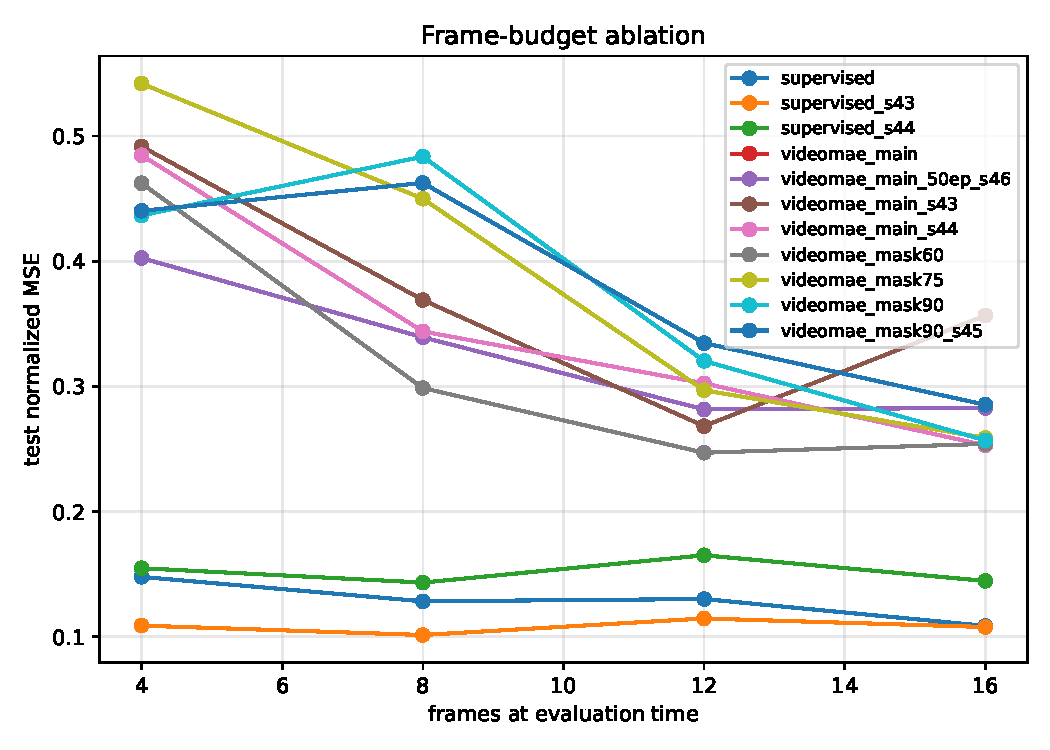
\includegraphics[width=0.49\textwidth,height=0.21\textheight,keepaspectratio]{frame_ablation.pdf}\hfill
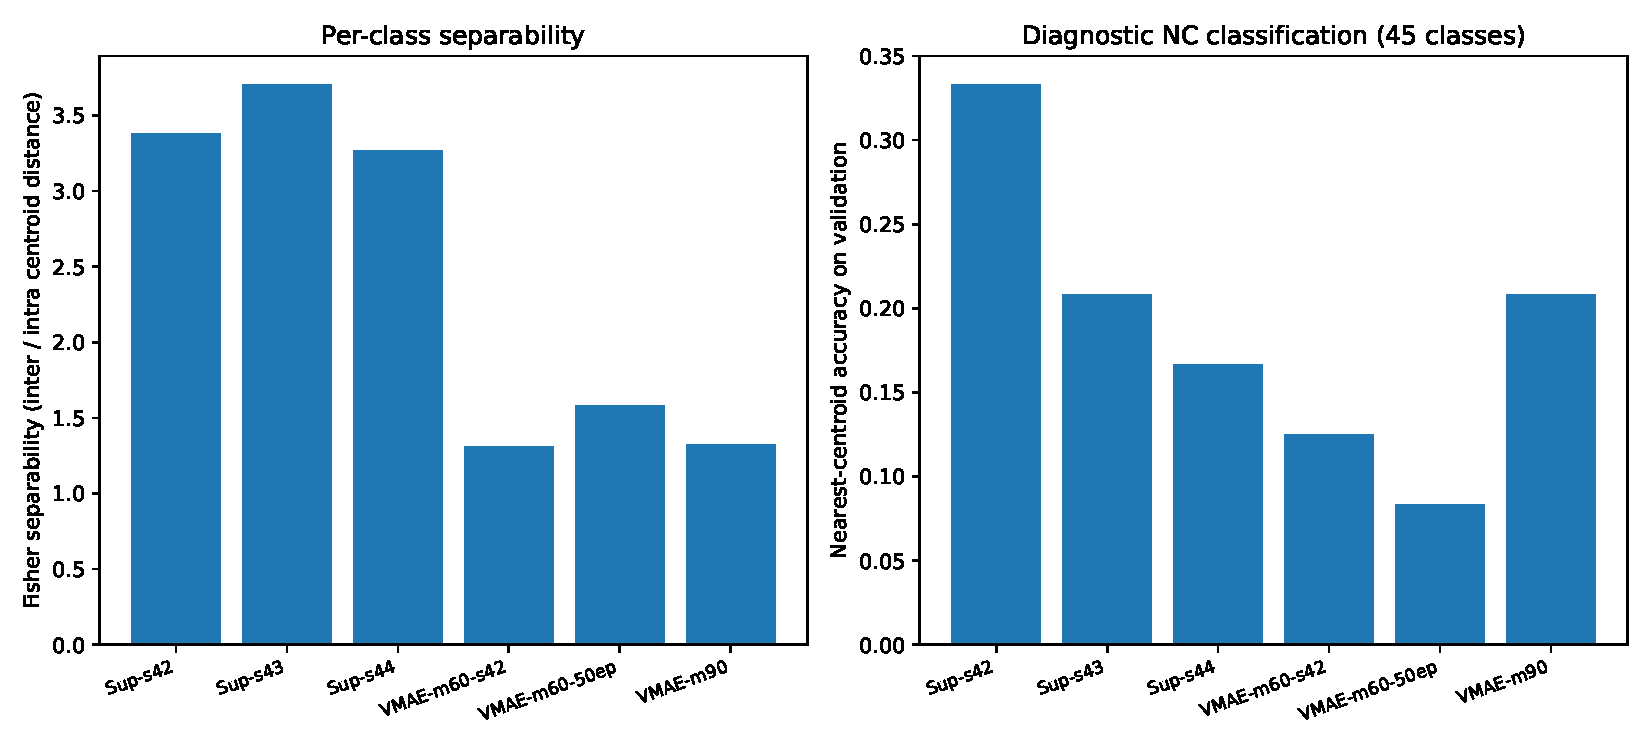
\includegraphics[width=0.49\textwidth,height=0.21\textheight,keepaspectratio]{class_separability.pdf}
\caption{Auxiliary diagnostics from supervised and VideoMAE-style masked-video probes, not used for final model selection. Left: masked-video encoders benefit from more temporal context at evaluation time. Right: nearest-centroid classification over the 45 $(\alpha,\zeta)$ combinations shows that stronger downstream regression aligns with stronger parameter-class separability.}
\label{fig:aux_diagnostics}
\end{figure*}

\section{Experiments}

\paragraph{Evaluation protocol.}
Each completed encoder is evaluated with the same downstream restrictions: frozen embeddings, one linear layer, and kNN regression. Hyperparameters are selected by validation normalized mean MSE. The final CNext embeddings are exported to \texttt{artifacts/emb\_cnext\_unet96\_avg/}. The selected linear probe uses z-scored features, learning rate $3\cdot10^{-3}$, weight decay 0, and effective full-batch training. The selected kNN uses z-scored features, Euclidean distance, uniform weighting, and $k=3$.

\begin{table*}[t]
\centering
\caption{Main frozen-encoder downstream results and auxiliary diagnostic probes. All MSE values are normalized by train-label statistics and evaluated on the held-out test split after validation-based selection. Auxiliary rows report mean MSE only and were not used as final submissions. Lower is better.}
\label{tab:results}
\resizebox{\textwidth}{!}{%
\begin{tabular}{llrrrr}
\toprule
Encoder / objective & Evaluator & Mean MSE & $\alpha$ MSE & $\zeta$ MSE & Notes \\
\midrule
CNext-U-Net forecasting & kNN & \textbf{0.0989} & \textbf{0.0121} & \textbf{0.1857} & final avg-pool export \\
CNext-U-Net forecasting & Linear & 0.1043 & 0.0371 & 0.1715 & required linear eval. \\
JEPA + VICReg & Linear & 0.2485 & 0.1183 & 0.3786 & original 224×224 baseline \\
JEPA + VICReg & kNN & 0.2709 & 0.0472 & 0.4946 & original 224×224 baseline \\
JEPA + VICReg (96×96) & Linear & 0.4260 & 0.1129 & 0.7391 & 96×96 rerun; sliding-window export \\
JEPA + VICReg (96×96) & kNN & 0.3865 & 0.2374 & 0.5356 & 96×96 rerun; $k{=}20$, cosine \\
ConvNeXt JEPA + SigReg & Linear & 0.5829 & 0.1872 & 0.9787 & SigReg loss frozen; export mismatch \\
ConvNeXt JEPA + SigReg & kNN & 0.5924 & 0.2058 & 0.9790 & SigReg loss frozen; export mismatch \\
\midrule
Supervised ConvNeXt probe & Direct reg. & 0.1090 & -- & -- & label-supervised diagnostic; seed 42 \\
Supervised ConvNeXt probe & Direct reg. & 0.1080 & -- & -- & label-supervised diagnostic; seed 43 \\
Supervised ConvNeXt probe & Direct reg. & 0.1450 & -- & -- & label-supervised diagnostic; seed 44 \\
VideoMAE-style masked video & Probe & 0.2540 & -- & -- & main masked-video diagnostic \\
VideoMAE-style masked video & Probe & 0.2830 & -- & -- & 50-epoch variant; seed 46 \\
VideoMAE-style masked video & Probe & 0.3570 & -- & -- & main variant; seed 43 \\
VideoMAE-style masked video & Probe & 0.2530 & -- & -- & main variant; seed 44 \\
VideoMAE-style masked video & Probe & 0.2540 & -- & -- & mask ratio 60\% \\
VideoMAE-style masked video & Probe & 0.2590 & -- & -- & mask ratio 75\% \\
VideoMAE-style masked video & Probe & 0.2570 & -- & -- & mask ratio 90\% \\
VideoMAE-style masked video & Probe & 0.2850 & -- & -- & mask ratio 90\%; seed 45 \\
\bottomrule
\end{tabular}
}
\end{table*}

\paragraph{Main results.}
Table~\ref{tab:results} summarizes both the eligible frozen-encoder runs and the auxiliary diagnostics. The CNext-U-Net encoder is best under both allowed downstream evaluators. Against the JEPA/VICReg baseline, it improves linear-probe mean MSE by 58\% relative ($0.2485 \rightarrow 0.1043$) and kNN mean MSE by 63\% relative ($0.2709 \rightarrow 0.0989$). The kNN gain is especially large on $\alpha$, where MSE drops from 0.0472 to 0.0121. CNext improves over the available JEPA/VICReg baselines, including a resolution-matched $96\times96$ rerun, though a fully controlled comparison would also match the downstream export protocol. CNext uses all train-split windows for self-supervised pretraining, but its downstream linear and kNN fitting uses the stricter trajectory-level protocol: one frozen embedding per train trajectory, or 175 labeled train embeddings. The JEPA exports use sliding-window downstream fitting, producing 11,550 train embeddings with repeated trajectory labels. The supervised and VideoMAE-style rows are included for completeness from the merged diagnostics; they support the same conclusion but are not final submissions because the supervised probes use labels and the masked-video probes underperform CNext.

\paragraph{Alpha versus zeta.}
Across all successful runs, $\zeta$ is harder than $\alpha$. For the final CNext model, kNN obtains $\alpha$ MSE 0.0121 but $\zeta$ MSE 0.1857. The same pattern appears in the baseline. We interpret this as evidence that visual signatures of active dipole strength are more directly reflected in short-horizon dynamics, while steric alignment may require longer temporal context or more global statistics. The final model still improves $\zeta$ relative to the JEPA baseline, reducing kNN $\zeta$ MSE from 0.4946 to 0.1857.

\paragraph{Auxiliary diagnostics.}
We also ran supervised and VideoMAE-style masked-video probes to understand the data geometry; these were trained from scratch on \texttt{active\_matter} and were not used as final frozen-encoder submissions because they underperformed the selected CNext forecaster. The frame-budget trend in Figure~\ref{fig:aux_diagnostics} supports using deterministic 16-frame trajectory clips for export, especially for masked-video encoders whose test MSE improves as more temporal context is available. The nearest-centroid diagnostic over the 45 $(\alpha,\zeta)$ combinations shows that better downstream regression coincides with stronger parameter-class separability, reinforcing that the task rewards embeddings organized by physical parameter geometry rather than pixel loss alone.

\section{Ablations and Failure Analysis}

\subsection{VICReg Avoided Collapse but Overfit Early}

The JEPA/VICReg baseline learned a healthy embedding space. The exported train embeddings had shape $11550\times128$, no dead dimensions under a standard deviation threshold of 0.01, and required 43 dimensions to explain 95\% of variance. This confirmed that VICReg's per-dimension variance and covariance penalties prevented collapse. However, training dynamics showed that the best validation checkpoint was early. Loss improved through epoch 5 and then validation loss increased, suggesting that the temporal prediction objective began overfitting or that the learning rate was too high for longer training. This was checkpoint selection on validation loss only; test labels were not used to choose epoch 5. This run was a strong baseline but not the final model.

A resolution-matched 96×96 rerun under the same hyperparameters and sliding-window export scored LP MSE $0.4260$ (vs.\ $0.2485$ at $224\times224$) and kNN MSE $0.3865$ (vs.\ $0.2709$). Reducing spatial resolution hurt JEPA substantially, likely because the JEPA prediction task relies on spatial structure that is captured more richly at higher resolution. Despite this degradation, CNext at $96\times96$ outperforms JEPA at both resolutions, confirming that the objective is the dominant factor in the improvement.

\subsection{SigReg Failed for Two Separate Reasons}

The SigReg run was intended to improve distance-based regression by making embeddings isotropic. Instead, it exposed two independent failures.

\textbf{Regularizer never activated.} Training finished, but \texttt{train\_sigreg\_loss} stayed frozen at 25.7268 and \texttt{valid\_sigreg\_loss} at 9.625 for all 25 epochs, unchanged from epoch 2 to epoch 25. \texttt{--target-stop-grad} fixed the trivial collapse, but the distribution term never got traction. The root cause: \texttt{pred\_loss} hit near-zero by epoch 2 (${\approx}9.7\times10^{-4}$) and the encoder locked into a local minimum. With \texttt{lejepa-lambda=0.05}, the SigReg gradient carried only 5\% of the total weight --- too weak to pull the encoder out once prediction was solved. The distribution regularization provided effectively zero gradient signal for the entire run. The result is an encoder trained purely on \texttt{pred\_loss}: a temporal prediction model that learned to map context$\to$target representations, but whose embedding distribution is not isotropic. The kNN benefit SigReg was supposed to provide did not materialize. The model is still notable --- at 9.83M parameters it is $3\times$ larger than the JEPA baseline and \texttt{pred\_loss} converged to ${\approx}7.5\times10^{-7}$ --- but not for the theoretical reasons intended.

\textbf{Export mismatch.} The downstream export used \texttt{single\_clip} mode: one deterministic embedding per trajectory, the same trajectory-level protocol the CNext model also uses. The JEPA baseline evaluation used sliding-window mode instead, producing 11,550 training embeddings --- one per overlapping window across all trajectories. That gives JEPA a large advantage in downstream training data and makes the comparison unfair in JEPA's favour. Both failures act simultaneously on the SigReg scores, making them invalid as a fair comparison against either model.

The embedding diagnostics agree with collapse: 62 of 256 dimensions had standard deviation below 0.01, and only 29 dimensions explained 95\% of variance. The model was larger than the baseline but used less of its representation space. This negative result changed the direction of the project: rather than increasing regularizer complexity, we moved to an objective with a stronger physical learning signal.

\subsection{Why Forecasting Worked Better}

The CNext-U-Net model predicts physical fields directly. This removes the shortcut where a predictor can match a moving latent target without preserving downstream-relevant information. Forecasting also exposes the encoder to the field variables at every spatial location, so the bottleneck must retain information about local patterns, temporal evolution, and global state. The decoder can be discarded after pretraining, leaving a compact encoder with a useful embedding geometry.

The pretraining history supports this interpretation. Validation relative MSE decreased from 0.1153 at epoch 1 to approximately 0.00252 at epoch 49, with no analogous frozen auxiliary term. The train and validation curves both decreased smoothly, indicating genuine learning rather than an early degenerate shortcut. The downstream gains show that forecasting did not merely solve pixel-level reconstruction; it produced embeddings that better organize the physical parameters.

\subsection{Pooling Ablation}

The final encoder produces a $672$-channel bottleneck map. We therefore tested whether downstream performance should use average pooling, max pooling, or their concatenation. Table~\ref{tab:pooling_ablation} reports both validation and test MSE for each pooling variant while keeping the encoder checkpoint, trajectory split, label normalization, and downstream search spaces fixed. Average pooling had the best validation MSE for both downstream evaluators and is therefore the selected final export. Max pooling achieved a slightly lower linear test MSE post hoc, but its validation MSE and kNN result were worse; selecting it on test performance would violate the validation-only model-selection protocol.

\begin{table}[t]
\centering
\caption{Pooling ablation for the final frozen CNext-U-Net encoder. Values are normalized mean MSE; pooling is selected by validation performance.}
\label{tab:pooling_ablation}
\resizebox{\columnwidth}{!}{%
\begin{tabular}{lrrrr}
\toprule
Pooling & Linear val & Linear test & kNN val & kNN test \\
\midrule
Avg only & \textbf{0.0593} & 0.1043 & \textbf{0.0240} & \textbf{0.0989} \\
Max only & 0.1073 & 0.0959 & 0.0981 & 0.1878 \\
Avg + max & 0.0886 & 0.1992 & 0.0612 & 0.1285 \\
\bottomrule
\end{tabular}
}
\end{table}

The pooling variants also clarify what the final geometry is using. Max pooling preserves peak local activations, which can make individual feature coordinates more sharply aligned with a linear decision surface and explains why max-only has the lowest linear test MSE post hoc. However, those peaks are less stable as a distance metric: kNN depends on neighborhood consistency across whole trajectories, and average pooling better preserves the global activity pattern that makes nearby embeddings share similar $(\alpha,\zeta)$. Average+max concatenation increases dimensionality but also adds noisy peak-sensitive coordinates, which hurt distance-based regression on the small trajectory-level validation and test sets.

\subsection{Representation Geometry}

Although the final pretraining task is next-frame forecasting, it is still representation learning because the downstream object is the frozen encoder bottleneck, not the decoder output. The physical parameters $\alpha$ and $\zeta$ control the evolution rule of the simulation, so predicting the next field from recent context requires the encoder to retain information about motion strength, alignment structure, and local interaction patterns. A representation that only memorizes instantaneous texture would be insufficient for low-error forecasting across trajectories with different dynamics.

We checked this geometry after training using only the train embeddings. After z-scoring final average-pooled CNext features, the first principal component had correlation $-0.971$ with normalized $\alpha$, while the second principal component had correlation $-0.881$ with normalized $\zeta$. This does not mean the model was trained with labels; it is a post-hoc diagnostic showing that the unlabeled forecasting objective arranged the frozen embeddings along axes aligned with the hidden physical parameters. The neighborhood structure also explains the large kNN gain: in train embeddings, the average normalized squared label distance among 5-nearest-neighbor pairs was 0.159, compared with 2.016 for random train pairs. The effect was strongest for $\alpha$ (0.024 local versus 2.015 random) and weaker but still clear for $\zeta$ (0.293 local versus 2.017 random). Thus, kNN improves because nearby CNext embeddings correspond to trajectories with similar physical parameters, not because the regressor has additional capacity.

\subsection{Embedding Health Check}

Table~\ref{tab:embedding_health} compares the same embedding diagnostics across the three main encoders. The CNext average-pooled embedding has many dimensions below the fixed 0.01 standard-deviation threshold, but this is partly a scale effect: its global feature standard deviation is only 0.0311, and no CNext dimension has standard deviation below $10^{-3}$. Therefore we interpret this as a compact low-amplitude trajectory representation rather than the SigReg failure mode, where poor downstream results, frozen regularization loss, and dead dimensions all appeared together.

\begin{center}
\captionsetup{hypcap=false}
\captionof{table}{Embedding health diagnostics on train embeddings. ``Dead dims'' uses a fixed per-dimension standard-deviation threshold of 0.01.}
\label{tab:embedding_health}
\resizebox{\columnwidth}{!}{%
\begin{tabular}{lrrr}
\toprule
Model & Dead dims & Dims for 95\% var & Global std \\
\midrule
JEPA/VICReg & 0/128 & 43/128 & 0.2237 \\
SigReg & 62/256 & 29/256 & 1.6230 \\
CNext-U-Net & 285/672 & 13/672 & 0.0311 \\
\bottomrule
\end{tabular}
}
\end{center}

\section{Compute Accounting and Artifacts}

\begin{center}
\captionsetup{hypcap=false}
\captionof{table}{Compute and artifact accounting. Earlier exploratory wall-clock logs were not retained, so exact GPU-hours are reported for the final run and configurations are listed for prior runs.}
\label{tab:compute}
\resizebox{\columnwidth}{!}{%
\begin{tabular}{@{}lll@{}}
\toprule
Run & Resource & Accounting \\
\midrule
JEPA/VICReg & $2\times$ A100, course HPC & 12 epochs; encoder + embeddings \\
JEPA/VICReg 96×96 & $2\times$ A100, course HPC & rerun; encoder + embeddings + eval \\
SigReg JEPA & $2\times$ A100, course HPC & 25 epochs; failure analysis \\
CNext-U-Net & $1\times$ B200, private cluster & 50 epochs; 0.48 GPU-h \\
Final eval. & $1\times$ B200, private cluster & $\sim$10 min; LP/kNN metrics \\
\bottomrule
\end{tabular}
}
\end{center}

The final CNext training log records 1726.89 seconds for 50 epochs, or 0.48 GPU-hours on one B200. Embedding export took approximately 3 minutes, the linear-probe sweep approximately 5 minutes, and the kNN sweep approximately 2 minutes. The committed artifacts include \texttt{encoder\_best.pt}, \texttt{encoder\_last.pt}, the training history and config JSON files, frozen train/validation/test embeddings, pooling-ablation embeddings and metrics, linear-probe weights and predictions, kNN predictions, and full training/evaluation logs. Larger optimizer-state checkpoints were intentionally not committed because they exceed common repository file-size limits; evaluation is reproducible from the committed frozen encoder.

\paragraph{Reproducibility note.}
All scripts set seed 42, but the final training config did not force deterministic cuDNN kernels. Exact weight-level reproduction may therefore require the same GPU and software stack, or a slower rerun with deterministic kernels enabled. The submitted checkpoint, exported embeddings, downstream configs, and saved predictions make the reported frozen-encoder evaluation reproducible without retraining.

\section{Limitations and Ethics}

The original JEPA/VICReg baseline used $224\times224$ frames; the final CNext model used $96\times96$ frames after TA clarification that the frame size may be changed. CNext improves over the available JEPA/VICReg baselines, including a resolution-matched $96\times96$ rerun, though a fully controlled comparison would also match the downstream export protocol. One remaining protocol difference is downstream export: both JEPA runs used sliding-window downstream fitting with 11,550 train embeddings that repeat trajectory labels, while CNext used trajectory-level fitting with 175 train embeddings.

Because downstream evaluation is trajectory-level, the final validation and test sets contain relatively few independent trajectories; therefore, the absolute MSE values should be interpreted alongside the consistent improvement across both linear probing and kNN.

The SigReg result should also be interpreted cautiously. It is valuable as a failure diagnosis, but the downstream numbers combine true representation collapse with an export-mode mismatch. We therefore do not treat SigReg as a competitive final model. Additionally, the task evaluates regression of two scalar physical parameters; strong performance does not imply that the representation captures all scientifically relevant active-matter phenomena.

Ethically, this work uses synthetic physical simulations rather than human data, so privacy risks are minimal. The main risk is scientific overclaiming: a low MSE on $\alpha$ and $\zeta$ should not be presented as a validated simulator, nor as evidence that the model has learned causal physical laws. Reproducible code, logs, and saved weights are included to make the reported claims auditable.

\section{Statement of Contributions}

Abhinay Krishna Bodi (ab11958) led the ConvNeXt JEPA encoder family, the JEPA/VICReg latent-prediction trainer (Sec.~4.1), the SigReg-regularized variant and its failure analysis (Sec.~4.2, Sec.~6.2), the resolution-matched 96$\times$96 JEPA rerun (Sec.~6.1), and the final CNext-U-Net forecaster (Sec.~4.4). Georgios Ioannou (gi2100) led the auxiliary supervised and VideoMAE-style masked-video diagnostic probes (Sec.~4.3), the channel-importance, frame-budget, and per-class separability analyses, and the cross-encoder CKA comparison.

We acknowledge the use of Claude Code and OpenAI Codex as programming and writing-assistance tools for code editing, experiment organization, and report drafting. All final technical decisions, validation, and submitted claims were reviewed and approved by the authors.

\section{Conclusion}

We evaluated self-supervised representation learning strategies for active-matter parameter regression under strict frozen-encoder downstream constraints. VICReg provided a stable non-collapsed baseline, while the SigReg attempt demonstrated that low prediction loss can mask a collapsed or poorly exported embedding space. The final CNext-U-Net forecaster gave the best representation, reaching normalized test MSE 0.1043 with a linear probe and 0.0989 with kNN. The main lesson is that, for this dataset, a direct physical forecasting objective produced more useful frozen embeddings than latent distribution regularization alone. CNext improves over the available JEPA/VICReg baselines, including a resolution-matched $96\times96$ rerun, though a fully controlled comparison would also match the downstream export protocol.

\bibliography{final_report_refs}
\bibliographystyle{icml2026/icml2026}

\end{document}
